\chapter{Estimativas de Custos}
\label{chapter:estimativa}

Para validar o baixo custo do sistema, este capítulo tem o foco em simular o orçamento de dois projetos. Um feito para a indústria e outro em redes domésticas para automações residenciais. Serão propostos cenários de aplicações reais, capazes de confirmar a premissa do projeto.
Como vimos no capítulo de projetos, o sistema pode ser instalado em plataformas mais sofisticadas, contendo sistemas operacionais e hardware dedicado. Mas nestes cenários utilizaremos o hardware mínimo que é compatível com o sistema e atua satisfatoriamente na aplicação.


\section{Aplicação: Automação Residencial}
\label{section:residencial}

O caso em estudo é a automação parcial de uma residência. Como pode ser visto em  \ref{fig:5.1.0/planta-casa}, a casa possui dois quartos, sala de estar, dois banheiros, cozinha, área de serviço e varanda. O objetivo é monitorar a temperatura local, o consumo de energia, detectar aberturas de portas e janelas de entrada da residência para fins de segurança e acionamento de luzes.

Para isso é necessário acionadores para a sala e cozinha, mais os quartos, totalizando cerca de 4 pontos de luz para acionar, o mesmo vale para os sensores de temperatura, no qual farão a média de temperatura da casa. Para controle de consumo de energia, nos limitaremos as tomadas de eletrodomésticos e eletrônicos, que representam a maior parte do consumo, para um ponto na sala, nos quartos, na tomada da geladeira, micro-ondas e lavadora, cerca de 6 tomadas a colocar sensores de tensão e corrente AC para cálculo da potência. Serão colocados sensores magnéticos para detectar abertura de portas e janelas, na porta de entrada, na porta da varanda, nas janelas do quarto e na área de serviço.

\begin{figure}[h!]
\centering
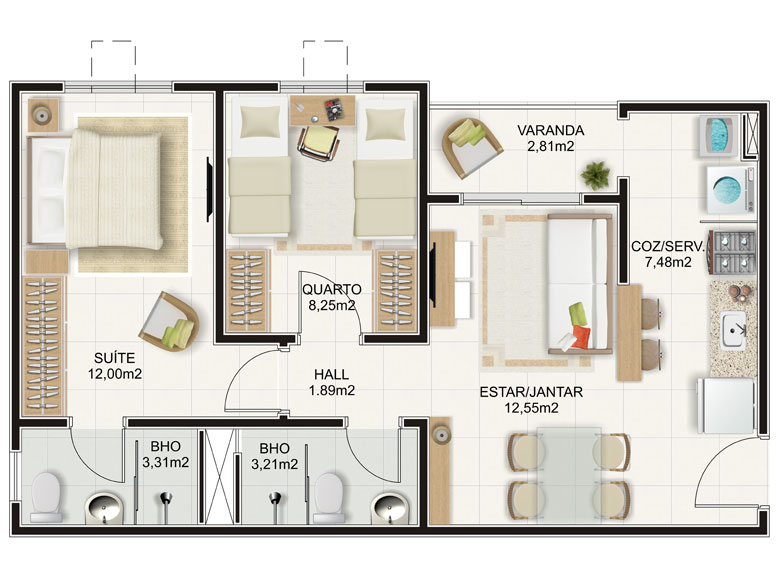
\includegraphics[width=13cm]{./02_Capitulos/02_Cap5/figures/planta-casa}
\caption{Planta baixa de residência de dois quartos, retirado de \cite{decorandocasas}}
\label{fig:5.1.0/planta-casa}
\end{figure}

Com menos de R\$ 2000,00 pode-se instalar um sistema robusto para automatizar uma casa. O projeto já conta que a residência possui uma rede WiFi e se a casa tiver um PC, pode-se abater do custo do servidor.


\begin{table}[h!]
\centering
\caption{Orçamento de um sistema simples para automação da residência da \ref{fig:5.1.0/planta-casa}}
\begin{tabular}{|l|l|l|l|l|}
\hline
Item                & Descrição                    & Qtde & Unidade (R\$) & Total (R\$) \\ \hline
esp32               & Módulo de aquisição          & 4    & \$30.00       & \$120.00    \\ \hline
DHT11               & Sensor de temperatura        & 4    & \$10.00       & \$40.00     \\ \hline
P8                  & Módulo sensor de tensão      & 6    & \$20.00       & \$120.00    \\ \hline
Acs712 - 5a         & Módulo sensor de corrente    & 6    & \$15.00       & \$90.00     \\ \hline
Ssr-25              & Relé Estado Sólido           & 4    & \$30.00       & \$120.00    \\ \hline
Desktop             & Servidor Local               & 1    & \$600.00      & \$600.00    \\ \hline
Sensores Magnéticos & Sensores de abertura         & 6    & \$40.00       & \$240.00    \\ \hline
Infraestrura        & Caixas de proteção, fios etc & 1    & \$500.00      & \$500.00    \\ \hline
\multicolumn{4}{|l|}{TOTAL:}                                              & \$1,830.00  \\ \hline
\end{tabular}
\label{table:planta-casa}
\end{table}

